%%%%%%%%%%%%%%%%%%%%%%%%%%%%%%%%%%%%%%%%%
% Original author:
% Linux and Unix Users Group at Virginia Tech Wiki
% (https://vtluug.org/wiki/Example_LaTeX_chem_lab_report)
% Modified by: Hector F. Jimenez S, for the Digital Electronics Laboratory.
% License:
% CC BY-NC-SA 3.0 
%%%%%%%%%%%%%%%%%%%%%%%%%%%%%%%%%%%%%%%%%
%----------------------------------------
%	PACKAGES AND DOCUMENT CONFIGURATIONS
%---------------------------------------
\documentclass[paper=a4, fontsize=12pt]{article} 		% A4 paper and 11pt font size
\usepackage[T1]{fontenc} 								% Use 8-bit encoding that has 256 glyphs
%\usepackage{fourier}		 							% Use the Adobe Utopia font for the document 
\usepackage[spanish,english]{babel}						% Spanish Language, templates uses some sections in english.
\selectlanguage{spanish}								% main language.
\usepackage{subfig}
\usepackage{multirow}
\PassOptionsToPackage{spanish}{babel}
\renewcommand{\figurename}{Figura}						% Force rename of figure.
\renewcommand{\figurename}{Fig.}
\usepackage[figurename=Fig.]{caption}
\usepackage[utf8]{inputenc}								% tildes for spanish language.
\usepackage{amsmath,amsfonts,amsthm} 					% Math packages.
\usepackage{minted}										% For syntax highlighting.
	    \renewcommand\listingscaption{Código}			%rename the source code minted !
\usepackage{float}										% Image will be in the same place as you want.!!! x-/
\usepackage{sectsty} 									% Allows customizing section commands
\allsectionsfont{\centering \normalfont\scshape}	   	% Make all sections centered, the default font and small caps
\usepackage{hyperref}
\hypersetup{											%Setups the false color and borders.
    colorlinks=false,
    pdfborder={0 0 0},
}
\newcommand\fnurl[2]{%									% set a simple and quick footnote command and include url.
\href{#2}{#1}\footnote{\url{#2}}%	
}
\usepackage{graphicx}									% Import easyly images.
\graphicspath{ {./images/} }							% Where to look for the images.
\DeclareGraphicsExtensions{.pdf,.png,.jpg}				% Graphics Extension to be used
\usepackage[notes,backend=biber]{biblatex-chicago}		% Bibliography and references.
\bibliography{biblio}									% bibliography filename.
\usepackage{fancyhdr} 									% Custom headers and footers
\pagestyle{fancyplain} 									% Makes all pages in the document conform to the custom headers and footers
\fancyhead{} 											% No page header
\fancyfoot[L]{} 										% Empty left footer
\fancyfoot[C]{} 										% Empty center footer
\fancyfoot[R]{\thepage} 								% Page numbering for right footer
\renewcommand{\headrulewidth}{0pt} 						% Remove header underlines
\renewcommand{\footrulewidth}{0pt} 						% Remove footer underlines
\setlength{\headheight}{13.6pt} 					    % Customize the height of the header
\numberwithin{equation}{section}						% Number equations within sections (i.e. 1.1, 1.2, 2.1, 2.2 instead of 1, 2, 3, 4)
%\numberwithin{figure}{section} 						% Number figures within sections (i.e. 1.1, 1.2, 2.1, 2.2 instead of 1, 2)
\numberwithin{table}{section} 							% Number tables within sections (i.e. 1.1, 1.2, 2.1, 2.2 instead of 1, 2, 3, 4)
\setlength\parindent{0pt} 								% Removes all indentation from paragraphs
\newcommand{\horrule}[1]{\rule{\linewidth}{#1}} 		% Create horizontal rule command with 1 argument of height
\usepackage{listings}% http://ctan.org/pkg/listings
\usepackage{multicol}
\usepackage{caption}
\usepackage{subfig}
\renewcommand{\lstlistingname}{Código}	
\title{Sistemas Operativos I\\ 
\horrule{0.5pt} \\[0.4cm] 								% Thin top horizontal rule	Title rule
\textit{Taller 2: Caso de estudio del sistema operativo Gnu/Linux, exploración superficial}
\horrule{1pt} \\[0.5cm] 			
} 			

\author{												
Héctor F. \textsc{Jiménez Saldarriaga.}\\				% Authors begin.
\texttt{hfjimenez@utp.edu.co} \\						
\texttt{PGP KEY ID: 0xB05AD7B8}
} 
% End of  Author name
\date{}    						                       % Date for the report, this will hide the \today.

\begin{document}
\maketitle                      			           % Insert the title, author and date
\begin{center}
\begin{tabular}{l r}								   % two column to
Fecha de Entrega: & Febrero, 2018 \\				   % Ramiro's Details.
Profesor: & Cesar Manuel Castillo Rodriguez
\end{tabular}
\end{center}
%%%%%%%%%%%	
% Let's start the document.
%%%%%%%%%%%	
\section{Objetivos}
\begin{itemize}
	\item Describir el proceso de instalación de un sistema operativo  Gnu\/Linux. 
    \item Realizar la identificación de la evolución del sistema operativo Gnu\/Linux.
    \item Realizar la identificación de la gestión de Procesos, Archivos, Shell.
    \item Identificar la estructura del Sistema Operativo.
    \item Clasificación del Sistema Operativo.
    \item Analizar el como se realiza el manejo de los dispositivos de entrada y salida.
    \item Interrupciones, como son en el sistema operativo actual. 
\end{itemize}
Este documento es el reporte del caso de estudio dedicado a los sistemas operativos Gnu/Linux, para este informe he decidido jugar con dos distribuciones de las cuales no tengo demasiado conocimiento que son Fedora, y CentOS. Explicare todos los detalles de basándome en el ultimo branch del kernel \textbf{\textit{4.14.20}}. 
La evolución de este sistema operativo trataré de explicarla con una perspectiva general, y no enfocada a una distribución en especifica.

El sistema operativo de un computador se puede definir, de una manera muy sencilla, como el software encargado de gestionar y manejar el hardware del equipo. Este creará una capa de abstracción sobre la complejidad de los circuitos y conexiones eléctricas que componen un computador proporcionando una interfaz amigable, pero si pensamos en todas las actividades que este gestiona para nosotros y somos conscientes de nuestra privacidad, y nuestra libertad en su uso debemos tener presente las opciones disponibles en el mercado, sus pros y sus contras. El kernel es una de las principales partes que componen todas las principales distribuciones GNU/Linux, normalmente esta pieza delicada y refinada del sistema operativo es desarrollado por voluntarios de todo el mundo, surgido en el año de 1990-1991 inicialmente como un proyecto universitario en la universidad de Helksinky. Alrededor del desarrollo del kernel se generaron una gran cantidad de distribuciones cada una con un enfoque diferente, algunas se especializan en una rama especifica de software otras simplemente tratan de ser independientes. Algunas veces a estas distribuciones se les llama sabores del ingles \textit{flavors}.
Hoy en día existen mas de 70 \fnurl{distribuciones }{https://en.wikipedia.org/wiki/List_of_Linux_distributions} cada una derivada de las distribuciones base :
\begin{multicols}{2}
\begin{enumerate}
\item \textbf{Debian-based}
\item CentOS/RHEL-based
\item Fedora-based
\item openSUSE-based
\item CentOS/RHEL-based
\item Fedora-based
\item openSUSE-based
\item Ubuntu-based
\item MEPIS-based
\item Knoppix-based
\item Pacman-based
\item Gentoo-based
\item Slackware-based
\item Mandrake/Mandriva-based
\end{enumerate}
\end{multicols}
\section{Proceso de instalación de un sistema operativo Gnu/Linux. }
Para realizar el proceso de instalación de un sistema operativo Gnu/Linux, inicialmente lo que necesitamos es tener una \textbf{\textit{motivación fuerte}} de probar otras formas filosóficas en las que se consume el software, teniendo en cuenta que utilizar un sistema operativo de cualquier distribución te brindará un control y poder total de las actividades que realiza el sistema, tendrás a disposición el código fuente si eres técnicamente hábil o si estas en el proceso de aprendizaje. Ambos sistemas operativos se encuentran basados en el uso de un gestor de paquetes definido por estándares de la compañía de red hat.
\subsection{Proceso de Instalación de Fedora}
\begin{figure}[H]
 	\centering
   	\subfloat[Seleccion Discos]{\label{fig:mdleft}{
   		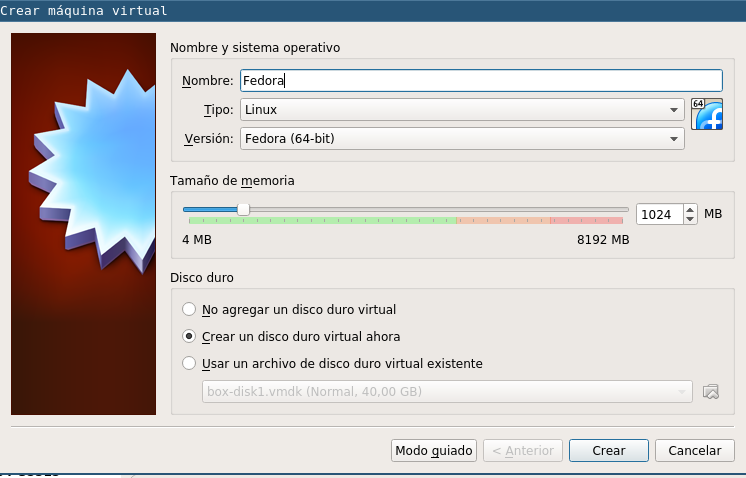
\includegraphics[width=0.45\textwidth]{img/discofedora1.png}
   		}}
	\subfloat[Carga instalador Fedora.]{\label{fig:mdleft}{
   		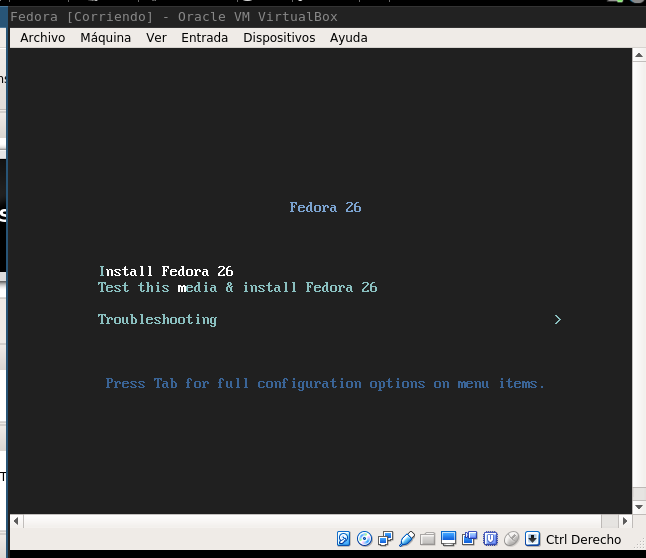
\includegraphics[width=0.35\textwidth]{img/disco2fedora.png}
        }}
       \hfill
	\subfloat[Seleccion de Idioma.]{\label{fig:mdleft}{
   		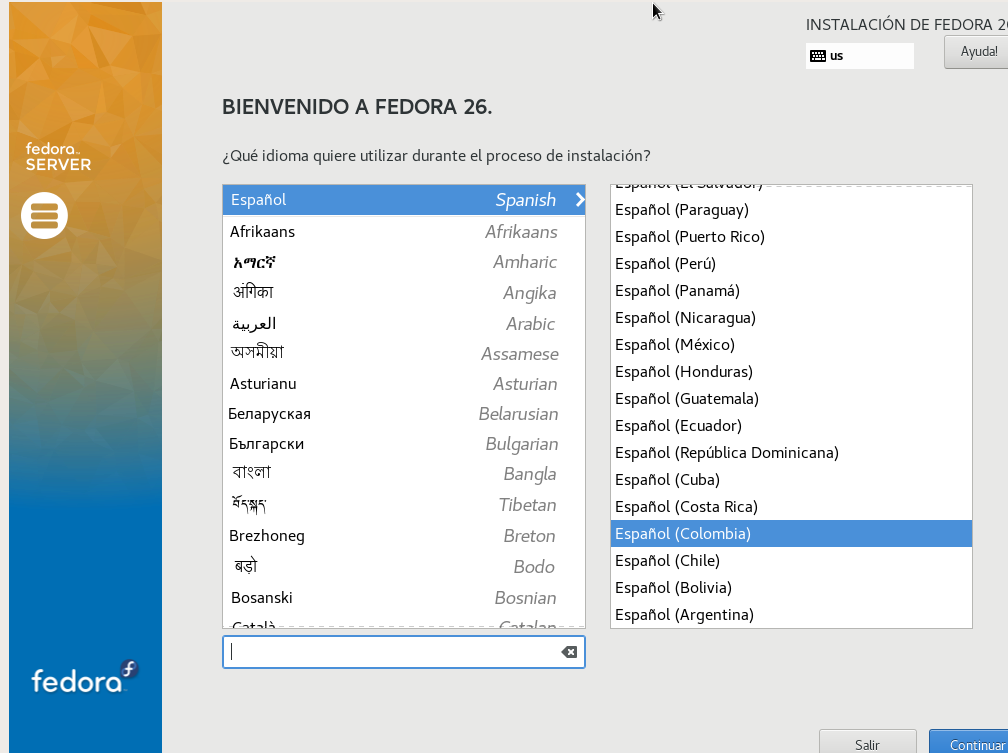
\includegraphics[width=0.45\textwidth]{img/disco3fedora.png}
        }}
	\subfloat[Parametros de Instalación.]{\label{fig:mdleft}{
   		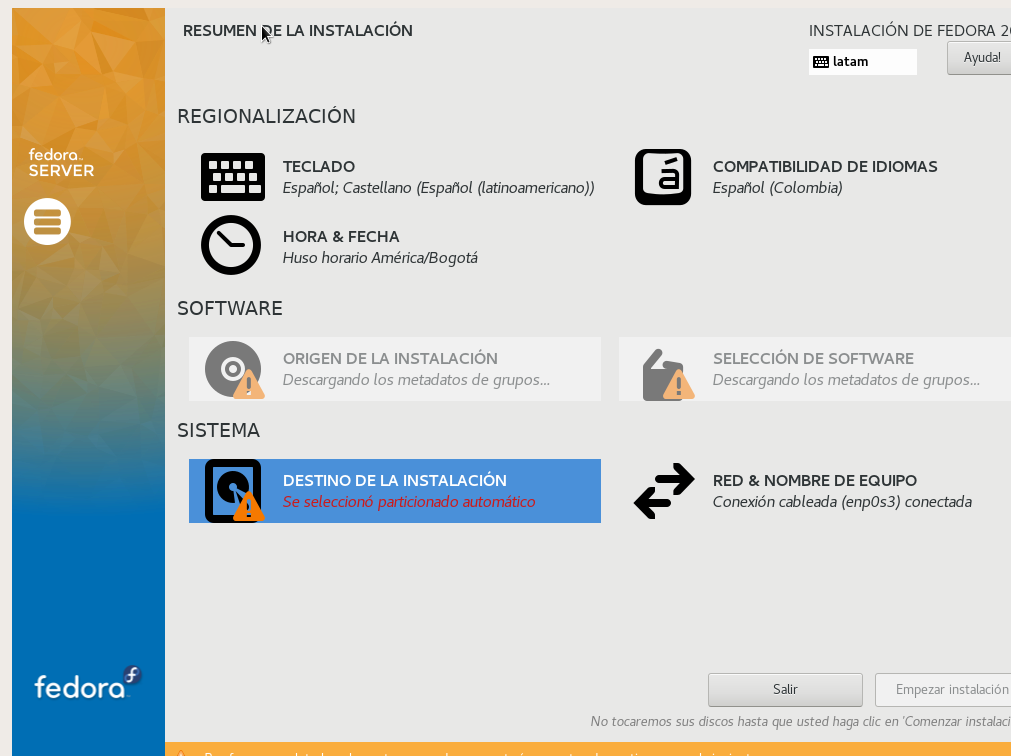
\includegraphics[width=0.45\textwidth]{img/disco4fedora.png}
        }}
\caption{Instalación de Fedora Gnu/Linux, Versión 26. Virtualbox}
\end{figure}
\subsection{Proceso de Instalación de CentOS}
\begin{figure}[H]
 	\centering
   	\subfloat[Seleccion Discos]{\label{fig:mdleft}{
   		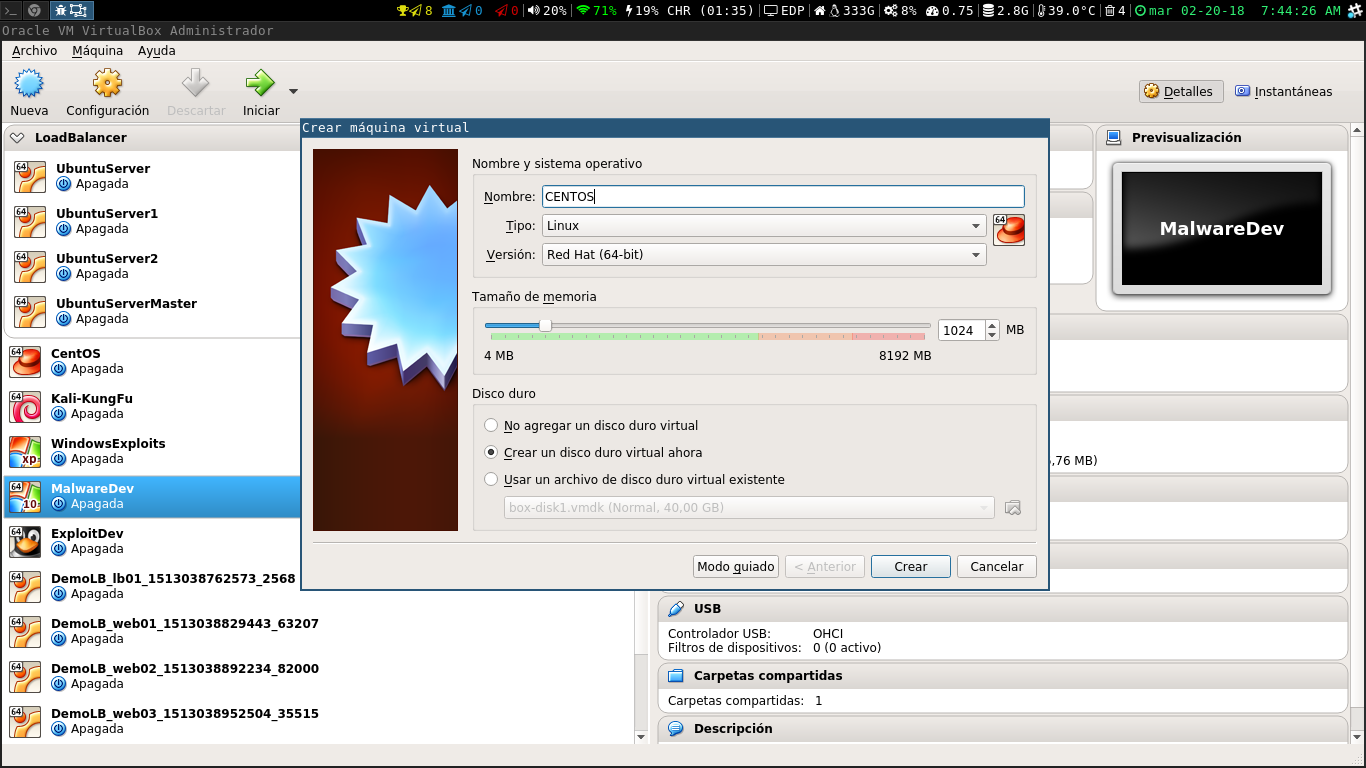
\includegraphics[width=0.4\textwidth]{img/1.png}
   		}}
	\subfloat[Configuración entorno para CentOS, similar en ambos.]{\label{fig:mdleft}{
   		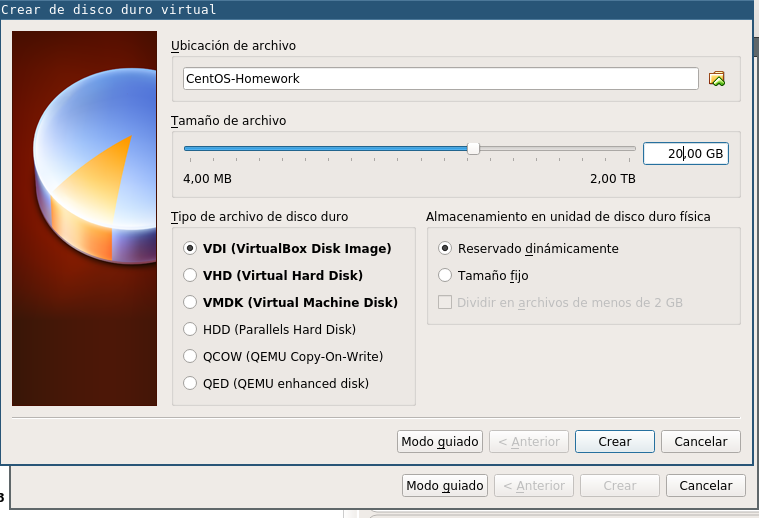
\includegraphics[width=0.4\textwidth]{img/2.png}
        }}
        \hfill
	\subfloat[Configuracion de maquina recien creada.]{\label{fig:mdleft}{
   		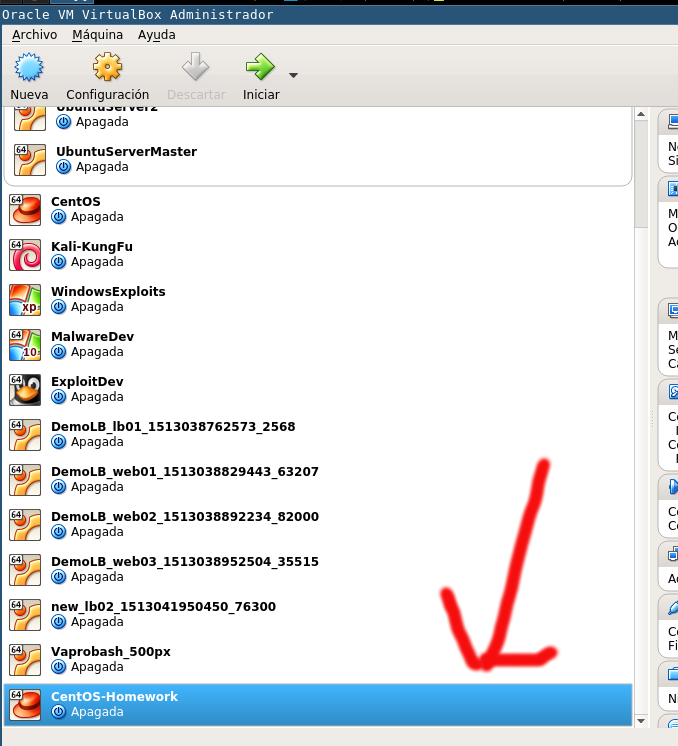
\includegraphics[width=0.4\textwidth]{img/3.png}
        }}
	\subfloat[Selección de imagen ISO, CentOS.]{\label{fig:mdleft}{
   		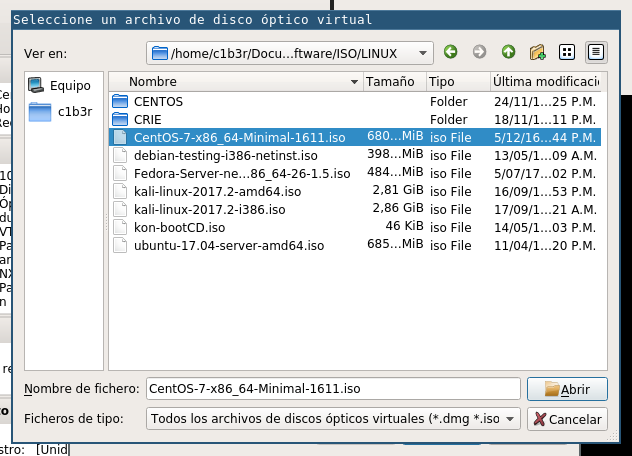
\includegraphics[width=0.4\textwidth]{img/4.png}
        }}
\caption{Instalación de CentOS Gnu/Linux. Virtualbox}
\end{figure}

\begin{figure}[H]
 	\centering
   	\subfloat[Párametros CentOS]{\label{fig:mdleft}{
   		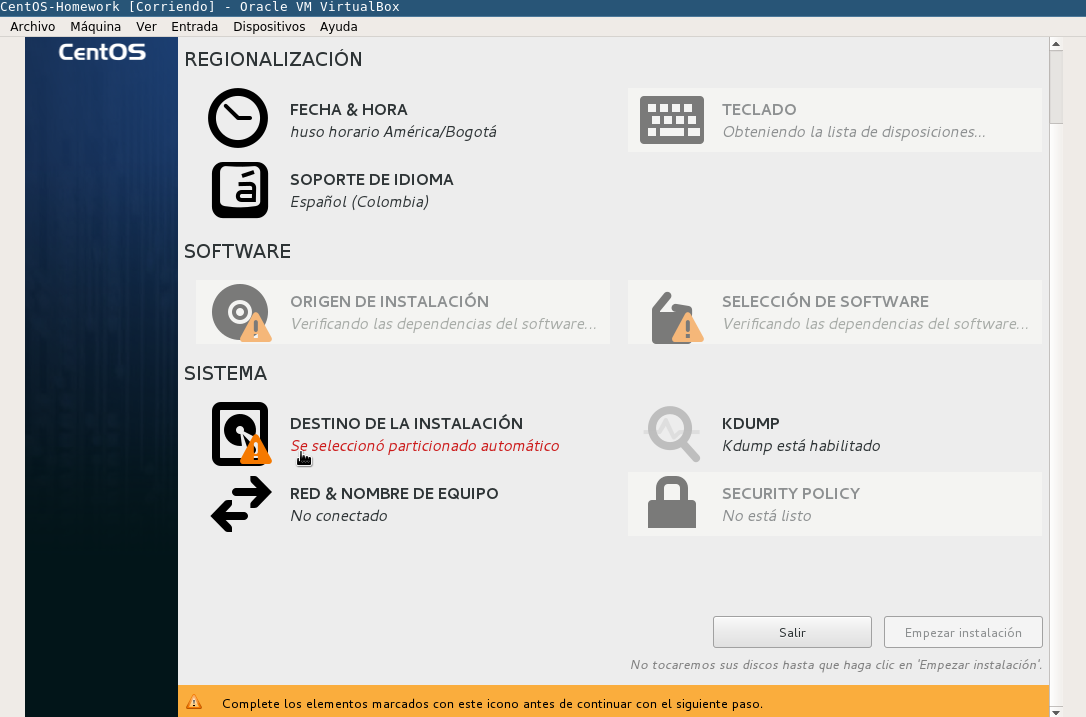
\includegraphics[width=0.4\textwidth]{img/5.png}
   		}}
	\subfloat[Selección particion vbox.]{\label{fig:mdleft}{
   		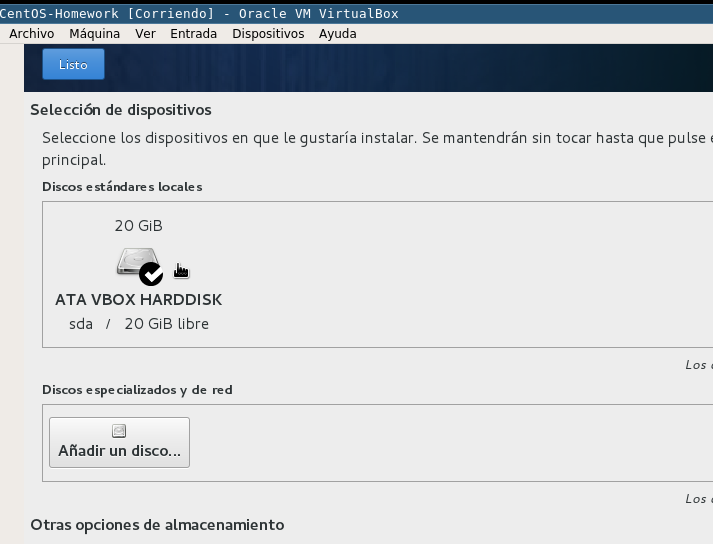
\includegraphics[width=0.4\textwidth]{img/6.png}
        }}
    \hfill
	\subfloat[Politicas de Seguridad.]{\label{fig:mdleft}{
   		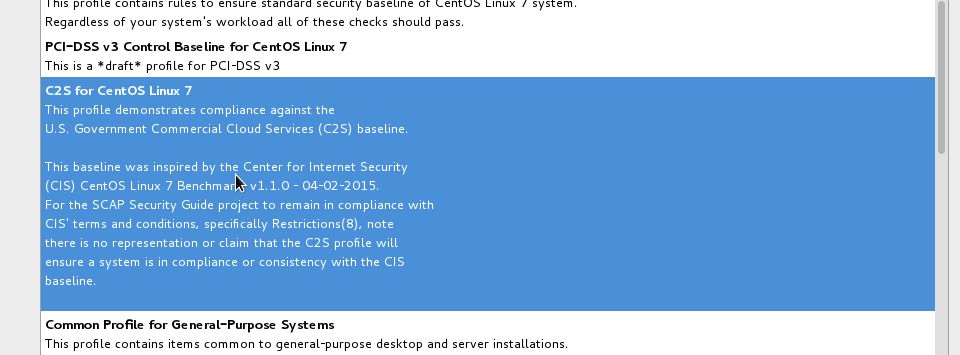
\includegraphics[width=0.4\textwidth]{img/7.png}
        }}
	\subfloat[Parametros de Instalación, Terminados.]{\label{fig:mdleft}{
   		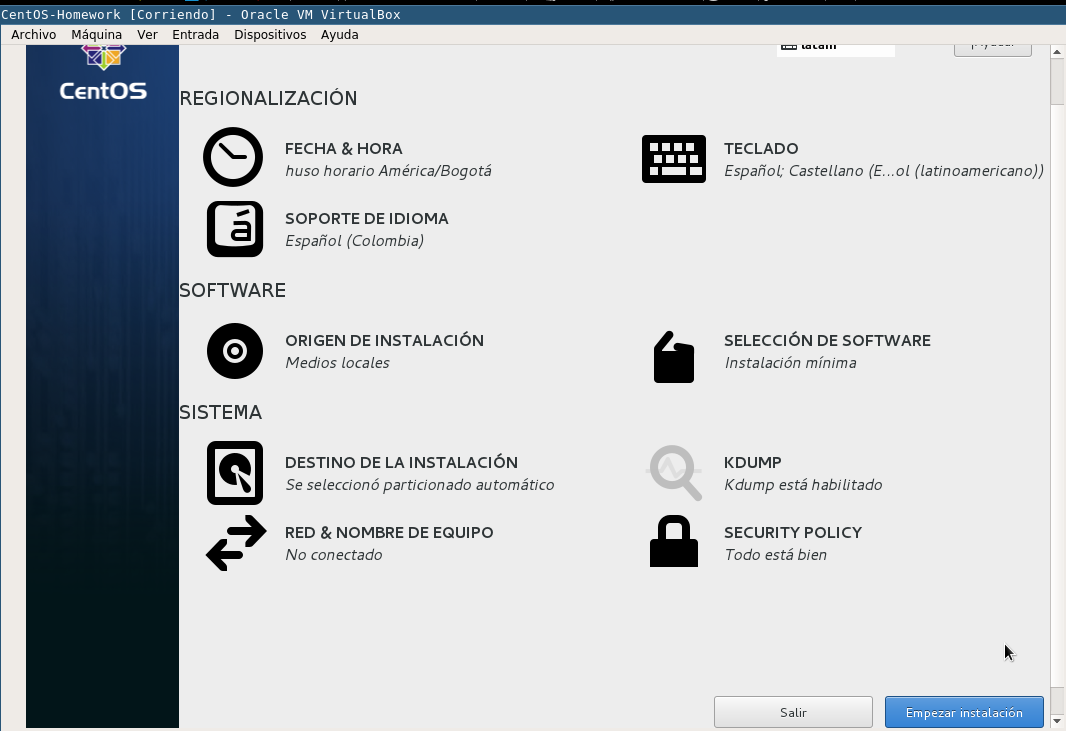
\includegraphics[width=0.4\textwidth]{img/8.png}
        }}
   \hfill
        \subfloat[Configuración usuario root.]{\label{fig:mdleft}{
   		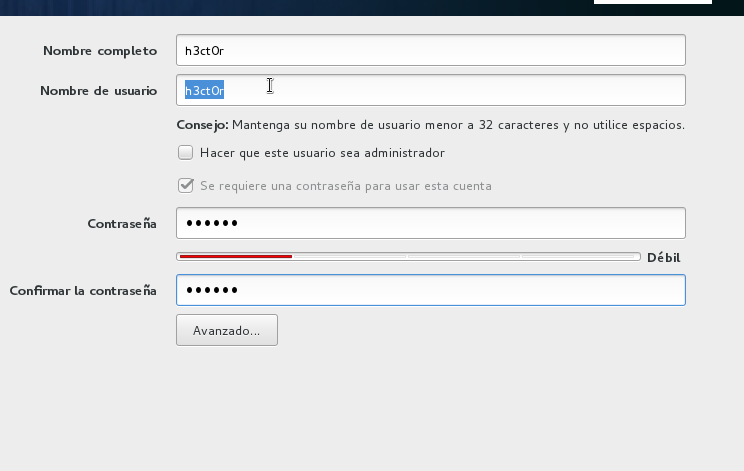
\includegraphics[width=0.4\textwidth]{img/9.png}
        }}
	\subfloat[Inicio proceso de instalación.]{\label{fig:mdleft}{
   		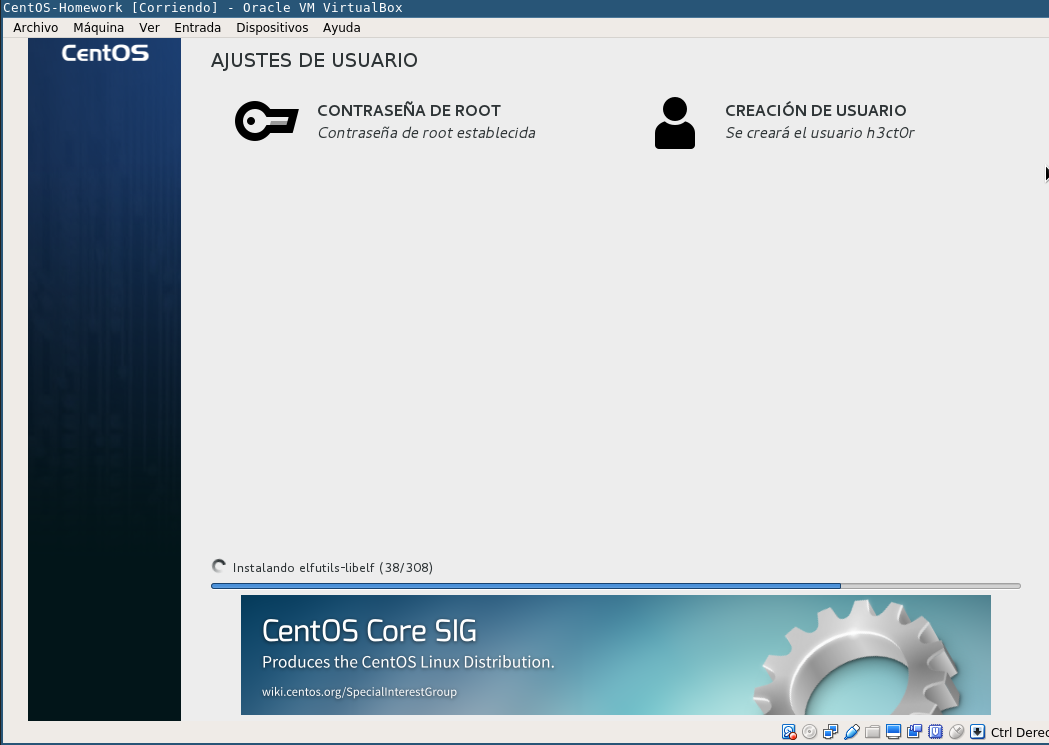
\includegraphics[width=0.4\textwidth]{img/10.png}
        }}
\caption{Proceso de instalación de CentOS Gnu/Linux. Virtualbox}
\end{figure}
Para realizar la instalación de ambos sistema operativos seguimos los pasos guiados indicados por el install wizard de cada sistema operativo, inicialmente se debe realizar la configuración de una nueva maquina virtual en nuestro virtualizador vbox, después seleccionamos la imagen ISO y la hacemos booteable, de esta forma el sistema arrancara por el cd de instalación. Ambas instalaciones lucen casi similares, la única diferencia encontrada entre ambas es que en el CENTOS al momento de realizar la instalación debía realizar la selección de una política de seguridad, la cual establecerá el nivel de control de acceso. 
Al explorar ambos sistemas operativos, como es claro ambos utilizan \textbf{yum} para la administración del software.
$$\\$$
\begin{itemize}
\item \textbf{yum} install \textit{packagename}
\item \textbf{yum} update \textit{packagename}
\item \textbf{yum} info \textit{packagename}
\item \textbf{yum} search \textit{packagename}
\end{itemize}
Una de las cosas también interesantes encontrada en este administrador de software es la agrupación, yo puedo realizar la agrupación de software similares, como por ejemplo servidores web, y solo actualizar ese grupo.
\section{Evolución del sistema operativo Gnu\/Linux.}	
Linux hace su aparición a principios de la década de los noventa, era el año \textbf{1991}, donde Linus Torvalds empezó como una afición a programar las primeras lineas de código de este sistema operativo al que llamaría más tarde Linux, apareciendo el 17 de  septiembre en algunos servidores \textit{ftp} disponibles.

El movimiento de software libre es iniciado por Richard Stallman para evitar que el laboratorio de inteligencia artificial del M.I.T. utilizara software privativo, luego extendió la idea a otras ramas del software de la época que en general era libre. 

En \textbf{1983} Rms crea el proyecto de GNU con el objetivo de crear un sistema operativo libre.
En \textbf{1989} Richard escribe la primera versión de la licencia GNU GPL \textbf{(V1.0)}
$$\\$$
Un resumen entorno a el desarrollo del kernel, es dado segun las versiones y series de este mismo encontrado en \fnurl{slideshare}{https://www.slideshare.net/OmarIsraellPB/evolucin-de-linux-14836584} \textbf{0.x} es a
\begin{description}
  \item[Serie \textbf{0.x}] \hfill \\ Se anuncia publicamente,algunos desarrolladores contribuyen mejoras y exntensiones para el mejor manejo de interrupciones. El nucleo se licencia bajo la licencia GPLV1.0. Mas de 100 desarrolladores implicados, adaptaciones al software usado por el proyecto GNU. Aparece la distribucion mas antigua Slackware, seguida de Debian. Actualmente Debian posee la comunidad mas grande de desarrolladores y usuarios, por encima de otras comerciales como ubuntu,suse.
  \item[Serie \textbf{1.x}] \hfill \\ Quizas el aporte mas grande fue el del contribuyente XFree86 Ccon su interfaz de usuario grafica. El kernel se porta a otras plataformas comerciales como DEC, Sun Sparc. Se define los modelos de manejo de versiones experimental, estable, current, y volatil. 
  \item[Serie \textbf{2.x}] \hfill \\ La versión 2.0 del núcleo Linux es liberada. Éste ahora puede servir varios procesadores al mismo tiempo, y así se hace una alternativa seria para muchas empresas.
  \begin{itemize}
  \item  Varios programas propietarios son liberados para Linux en el mercado, como la base de datos Adabas D, el navegador Netscape y las suites de oficina Applixware y StarOffice
  \item Empresas importantes de informática como IBM, Compaq y Oracle anuncian soporte para Linux.
  \item El proyecto KDE ve la luz, en su idea por mejorar las interfaces de usuario. 
  \item Soporte para transporte de datos de red, protocolo SMP. 
  \item Aparece el competidor numero 1 de KDE, GNOME. 
  \item Aparece una suite ofimatica mas avanzada que todas las presentes en el mercado, StarOffice. 
  \end{itemize}
  \item[Serie \textbf{3.x}] \hfill \\Enero de 2001, se libera la serie 2.4 del núcleo Linux. El núcleo Linux ahora soporta hasta 64 Gb de RAM, sistemas de 64 bits, dispositivos USB y un sistema de archivos \fnurl{journaling}{que es journaling, descripcion en ingles http://www.linfo.org/journaling_filesystem.html}.
  \begin{itemize}
  \item  El equipo de XFree86 se desintegra y se forma la fundación X.Org, que provoca un desarrollo considerablemente más rápido del servidor X para Linux
  \item Red Hat permiten el uso de efectos acelerados por hardware sobre el escritorio Linux.
  \item Dell llega a ser el primer fabricante principal de computadoras en vender una computadora personal de escritorio con Ubuntu pre instalado.
  \end{itemize}

  \item[Serie \textbf{4.x}] \hfill \\ Esta seria se piensa mas en el uso de  todo tipo de dispositivo, mas hacia moviles. Importantes mejoras surgen en  el tema del sandboxing y aislamiento de procesos, programas. Se permite multiples operaciones IO, mejora de concurrencia y soporte para hardware actual del mercado. 
\end{description}
\begin{figure}[H]
 	\centering
   	\subfloat[Arquitectura de  Contribuciones Kernel,resumen yocto.]{\label{fig:mdleft}{
   		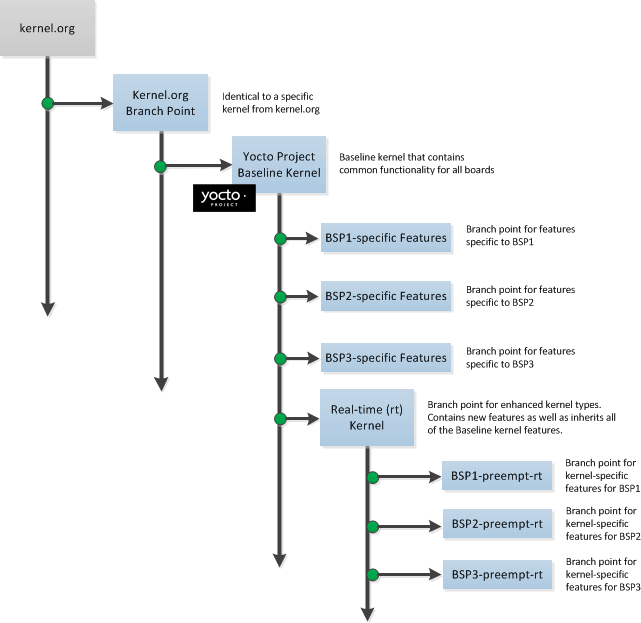
\includegraphics[scale=0.4]{img/kernelarch.png}}}
\end{figure}
\section{Clasificación del Sistema Operativo.}
Según el libro de sistemas operativos estos pueden ser clasificados de acuerdo a :
\begin{itemize}
\item\textbf{Multiusuario}: Permite que dos o más usuarios utilicen sus programas al mismo tiempo. Algunos sistemas operativos permiten a centenares o millares de usuarios al mismo tiempo.
\item\textbf{Multiprocesador}: soporta el abrir un mismo programa en más de una CPU.
\item\textbf{Multitarea}: Permite que varios programas se ejecuten al mismo tiempo.
\item\textbf{Multitramo}: Permite que diversas partes de un solo programa funcionen al mismo tiempo.
\item\textbf{Tiempo Real}: Responde a las entradas inmediatamente. 
\end{itemize}
Todas las distribuciones Gnu/Linux actualmente soportan la gran mayoría de items descritos en el libro mencionado del señor Tanembaum.
\section{Identificación de la gestión de Procesos, Archivos, Shell.}
\subsection{Sistema de Archivos}
Un sistema de archivos es una forma de almacenar información en un computador de forma persistente, normalmente consiste de una estructura jerárquica de archivos, a esto también se le conoce como árbol de directorios. Cada dispositivo de almacenamiento persistente y a su vez sus particiones pueden tener cualquier sistema de archivo por elección. En los sistemas operativos Gnu/Linux tenemos sistemas de archivos con Journaling, que es una previsión de pérdida de datos por fallos del disco o apagones. En contra prestación, es totalmente imposible recuperar datos borrados. 
El journaling permite generar una especie de foto del estado de los datos de escritura en los discos, esta copia se realiza sobre los metadatos de los archivos presentes en el sistema de archivo, luego puede ser restaurada por el sistema operativo, todo ello gracias a la cooperación que hay entre las funciones que tiene el kernel y los dispositivos de almacenamiento.
Linux soporta gran variedad de sistemas de ficheros actualmente, desde sistemas basados en discos, como pueden ser \textbf{ext2, ext3, ReiserFS, XFS, JFS, UFS, ISO9660, FAT, FAT32 o NTFS}, a sistemas de ficheros que sirven para comunicar equipos en la red de diferentes sistemas operativos, como \textbf{NFS} (utilizado para compartir recursos entre equipos Linux) o \textbf{SMB} (para compartir recursos entre máquinas Linux y Windows)
En todas las distribuciones  Gnu/Linux tenemos un esquema jerárquico como se menciono previamente donde cada archivo y carpeta dentro del sistema tiene una propuesta importante. 
\begin{figure}[H]
 	\centering
   	\subfloat[Estructura de un sistema de archivo Gnu/Linux Debian 10.]{\label{fig:mdleft}{
   		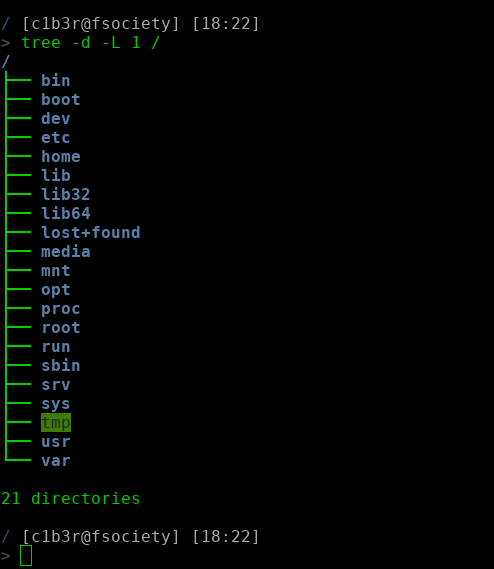
\includegraphics[scale=0.4]{img/structura.png}}}
\end{figure}
\subsection{Gestion de Procesos}
Cada programa que se ejecuta es un proceso con recursos asignados y gestionado por el kernel. La gestión de procesos comprende el  monitoreo, detención y cambio de prioridad de los procesos. normalmente esto lo realiza el sistema operativo sin nuestra intervención, pero algunas veces por circunstancia necesitaremos intervenir.

Un proceso el cualquier distribución linux sigue los estándares LSB, para los cuales se tienen  los siguientes parámetros :
\begin{itemize}
\item PROCESS ID (PID): Numero entero identificador del proceso
\item USER ID, GROUP ID: Todos los procesos tiene asociado un usuario y grupo en la escala de privilegios
\item PARENT PROCESS: Proceso padre del proceso.
\item ENVIROMENT:lista de variables utilizada por el proceso.
\item CURRENT WORKING DIRECTORY: directorio de ubicación del ejecutable asociado al proceso.
\item NICE NUMBE: prioridad de ejecución de los procesos, permite dar mas prioridad del uso de la cpu.
\end{itemize}
Cada uno de los parámetros puede ser seguido de manera cuidadosa, esto permite establecer y rastrear acciones maliciosas realizadas por procesos dentro del sistema.
En un entorno Unix, Linux tenemos multiples herrramientas que nos permiten analizar y gestionar los procesos, a continuacion una lista: 
\begin{enumerate}
\item htop, mi favorito tiene colores e indicadores. Atajos rapidos.
\item ps, la herramienta universal  integrada con cada distribucion. 
\item atop, herramienta mas detallada
\end{enumerate}


\begin{figure}[H]
 	\centering
   	\subfloat[Herramienta Htop, colores e indicadores.]{\label{fig:mdleft}{
   		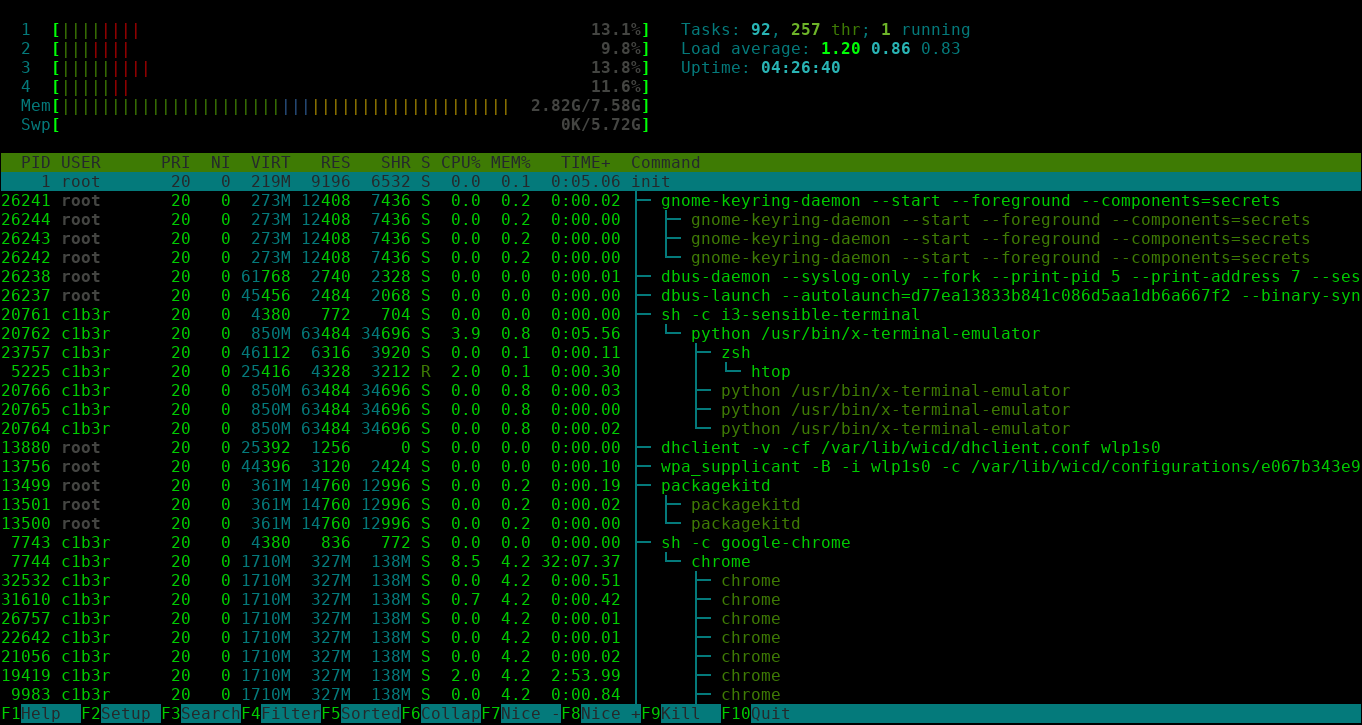
\includegraphics[scale=0.3]{img/htop.png}
   		}}
        \vfill
	\subfloat[resumen ligero.]{\label{fig:mdleft}{
   		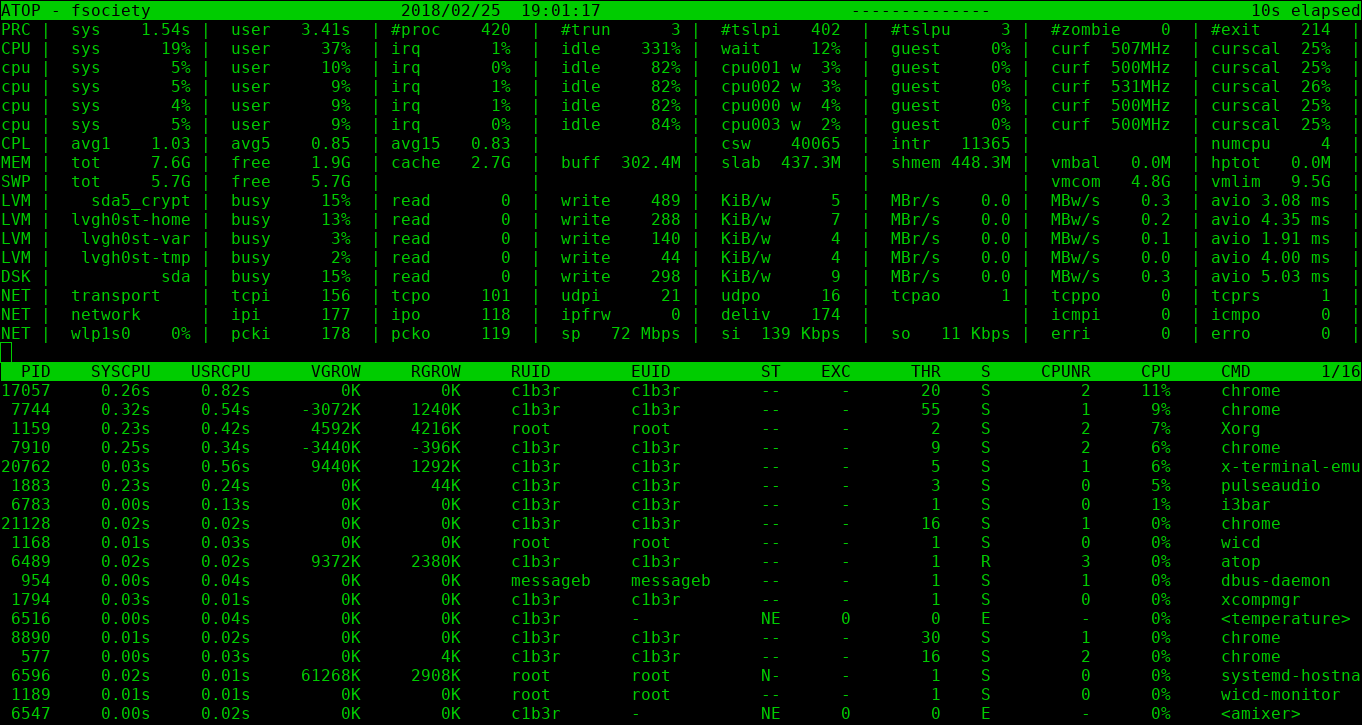
\includegraphics[scale=0.3]{img/atop.png}
        }}    
\caption{Herramientas para la gestión de procesos}
\end{figure}

\section{Estructura del Sistema Operativo.}
\begin{figure}[H]
 	\centering
   	\subfloat[Llamadas Sistema, interacion entre capas]{\label{fig:mdleft}{
   		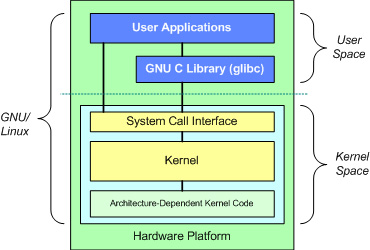
\includegraphics[scale=0.4]{img/kernelh.jpg}}}
\end{figure}
\section{Manejo de dispositivos de entrada y salida.}
\begin{figure}[H]
 	\centering
   	\subfloat[Dispositivos de ejecución estándar, std-in, std-out, std-err]{\label{fig:mdleft}{
   		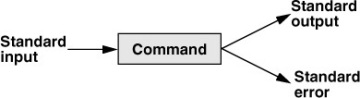
\includegraphics[scale=0.6]{img/devices.jpg}}}
\end{figure}
\section{Referencias}
\begin{itemize}
\item  \hyperref[http://www.linfo.org/index.html]{The Linux Information Project,  http://www.linfo.org/index.html}
\item  \hyperref[http://kernel.org]{Kernel Development,  http://www.kernel.org}
\item  \hyperref[http://www.linfo.org/journaling_filesystem.html]{Journaling Filesystem Definition, http://www.linfo.org/journaling\_filesystem.html}
\item  \hyperref[http://www.informit.com/articles/article.aspx?p=2273593&seqNum=5]{Standard Input and Standard Output, http://www.informit.com/articles/}
\end{itemize}
\end{document}